 
% Para una visualizacion correcta, generar el PDF
% Ni el DVI ni el PS se visualizan bien

% Elegir el estilo que se desee, hay cientos en la red

\documentclass{beamer}
\usepackage{beamerthemeshadow}
%\usepackage[galician]{babel}
\usepackage[spanish]{babel}
\usepackage[utf8]{inputenc}
%\usepackage[latin1]{inputenc}

\begin{document}
\title{Paralelización del algoritmo Progressive Hedging para la resolución de problemas estocásticos}
\subtitle{Grao en Ingeniería Informática \\
Universidad de Santiago de Compostela}  
\author{Autor: Cristofer Canosa Domínguez}
\institute{Director: Juan Carlos Pichel Campos}
\date{\today} 

\begin{frame}
\titlepage
\end{frame}

\begin{frame}
\frametitle{Tabla de contenidos}
\tableofcontents
\end{frame} 

\section{Introducción}

\subsection{Programación Estocástica}

\begin{frame}
    \frametitle{Programación estocástica}
    \begin{itemize}
        \item Problemas de optimización \pause
        \item Existe un nivel de incertidumbre \pause
        \item Generan múltiples escenarios
    \end{itemize}
\end{frame}

\begin{frame}
    \frametitle{Programación estocástica}
    \begin{figure}[H]
        \centerline{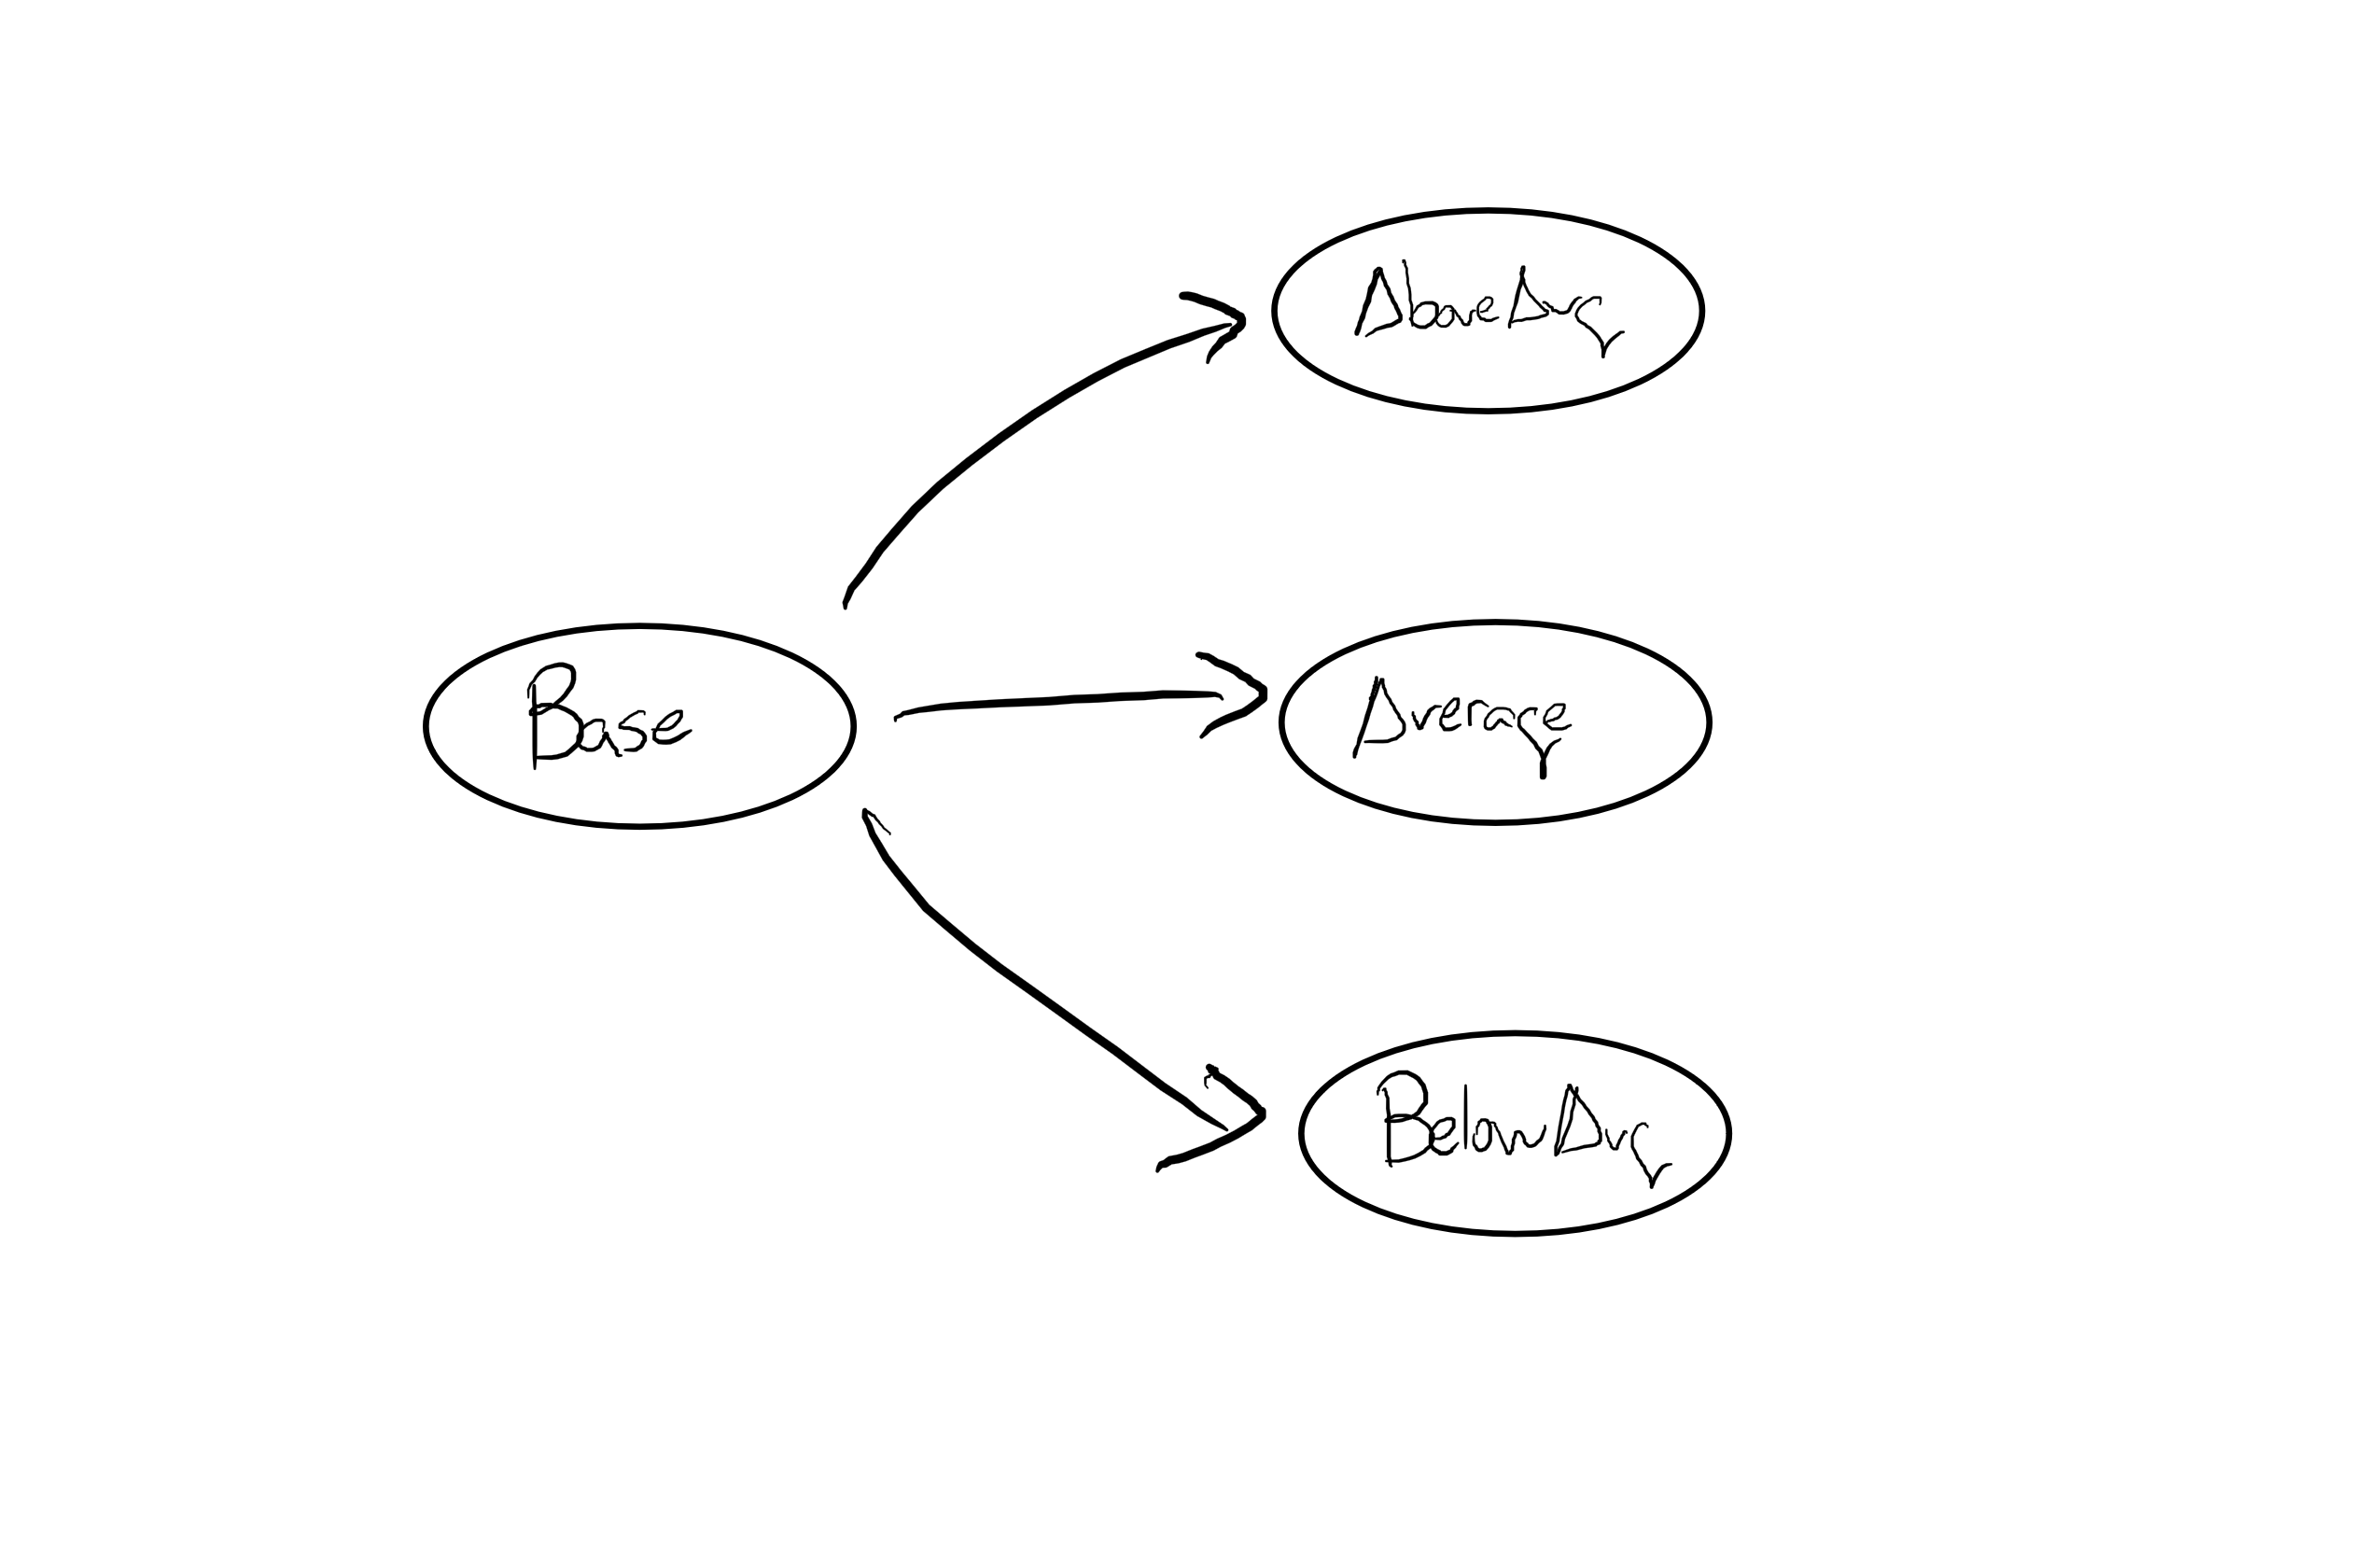
\includegraphics[width=8cm]{figuras/scenario-tree.png}}
        \caption{Árbol de escenarios en un problema estocástico}
        \label{fig:scenario-tree}
    \end{figure}
    % Explicar que son las variables las que generan los múltiples escenarios. Si tenemos más de una variable, el árbol crece.
\end{frame}

\begin{frame}
    \frametitle{Ejemplos de aplicación}
    \begin{enumerate}
        \item TFM: ``Problemas de rutas de vehículos''
        % Abastecer a un conjunto de clientes con un número concreto de vehículos. Se busca la ruta óptima. Múltiples puntos de salida. Se diferencia del problema del viajante en que cada vehículo tiene una capacidad concreta. p.e si tenemos repartidores de pizzas: cuantas pizzas puede llevar cada coche.
        % Incertidumbre en la demanda.
        \item Modelo de optimización de la oferta de generación eléctrica para compañías eléctricas que participan en el mercado eléctrico liberalizado MIBEL.
        % MIBEL: Mercado Ibérico de la Electricidad.
        % Grupo de mercado en el que las compañías generadoras ofertan energía y los distribuidores realizan una demanada.
        \item ``Progressive Hedging aplicado a coordinación hidrotérmica''
        % Optimizar una red eléctrica con múltiples fuentes de energía y la variabilidad que introducen.
    \end{enumerate}
\end{frame}

\subsection{Pyomo}

\begin{frame}
    \frametitle{Pyomo}
    \begin{columns}
        \begin{column}{5cm}
            \begin{itemize}
            \item Formulación y solución de modelos de optimización
            \item Uso de solucionadores de terceros (CPLEX, GLPK)
            \item \textit{Sandia National Laboratories} y \textit{University of California}
            \item Python
            \end{itemize}
        \end{column}
        \begin{column}{5cm}
            \begin{figure}[H]
                \centerline{
\includegraphics[width=3cm]{figuras/pyomo-logo.png}}
            \end{figure}
        \end{column}
    \end{columns}
    % Programa de código abierto que se usa para solucionar problemas de optimización de todo tipo. Permite escribir un script en python que defina tu problema y lo soluciona. 
    % Usa los solvers de terceros. Existe una interfaz muy conocida AMPL.
    % Nos centraremos en PySP que es el módulo concreto orientado a la resolución de problemas estocásticos.
\end{frame}

\subsection{Objetivos}

\begin{frame}
    \frametitle{Objetivos}
    \begin{enumerate}
        \item Estudiar y analizar el funcionamiento del algoritmo \textit{Progressive Hedging} en PySP.
        \item Análisis de las diferentes alternativas de paralelización disponibles que mejor se adapten al problema. Se tendrán en cuenta tecnologías Big Data (Apache Spark) o modelos tradicionales de paralelización.
        \item Diseño e implementación del nuevo módulo e integración con Pyomo.
        \item Análisis y evaluación del rendimiento.
    \end{enumerate}
\end{frame}

\section{Gestión del proyecto}

\subsection{Alcance y entregables}

\begin{frame}
    \frametitle{Alcance}
    \begin{itemize}
        \item Adaptar el módulo de programación estocástica (PySP) a una nueva implementación paralela.
        \item Nueva implementación más escalable que permita abordar problemas de mayor tamaño.
        \item Realizar un análisis de rendimiento.
    \end{itemize}
\end{frame}

\begin{frame}
    \frametitle{Entregables}
    \begin{itemize}
        \item Código de Pyomo actualizado con el módulo de ejecución de PH paralelo.
        \item Estudio de rendimiento.
        \item Memoria de realización del proyecto.
        \item Otra documentación asociada a la realización del proyecto.
    \end{itemize}
\end{frame}

\begin{frame}
    \frametitle{Casos de uso}
    \begin{figure}[H]
        \centerline{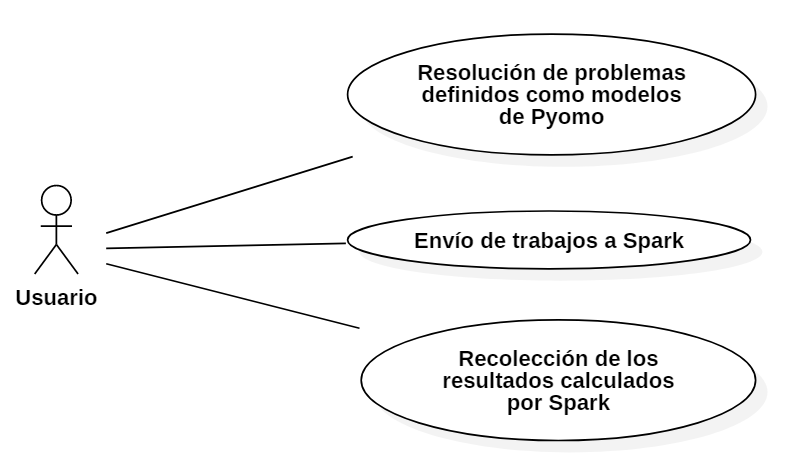
\includegraphics[width=8cm]{figuras/analisis/use-cases.png}}
        \caption{Casos de uso}
        \label{fig:use-cases}
    \end{figure}
\end{frame}

\subsection{Planificación temporal}

\begin{frame}
    \frametitle{Metodología de desarrollo}   
    \begin{itemize}
        \item Límite temporal estricto \pause
        \item Poco peso de la fase de implementación \pause
        \item Mayor énfasis en análisis y documentación \pause
        \item Metodología en cascada
    \end{itemize} 
\end{frame}

\begin{frame}[plain]
    \frametitle{EDT}
    \begin{figure}[H]
        \centerline{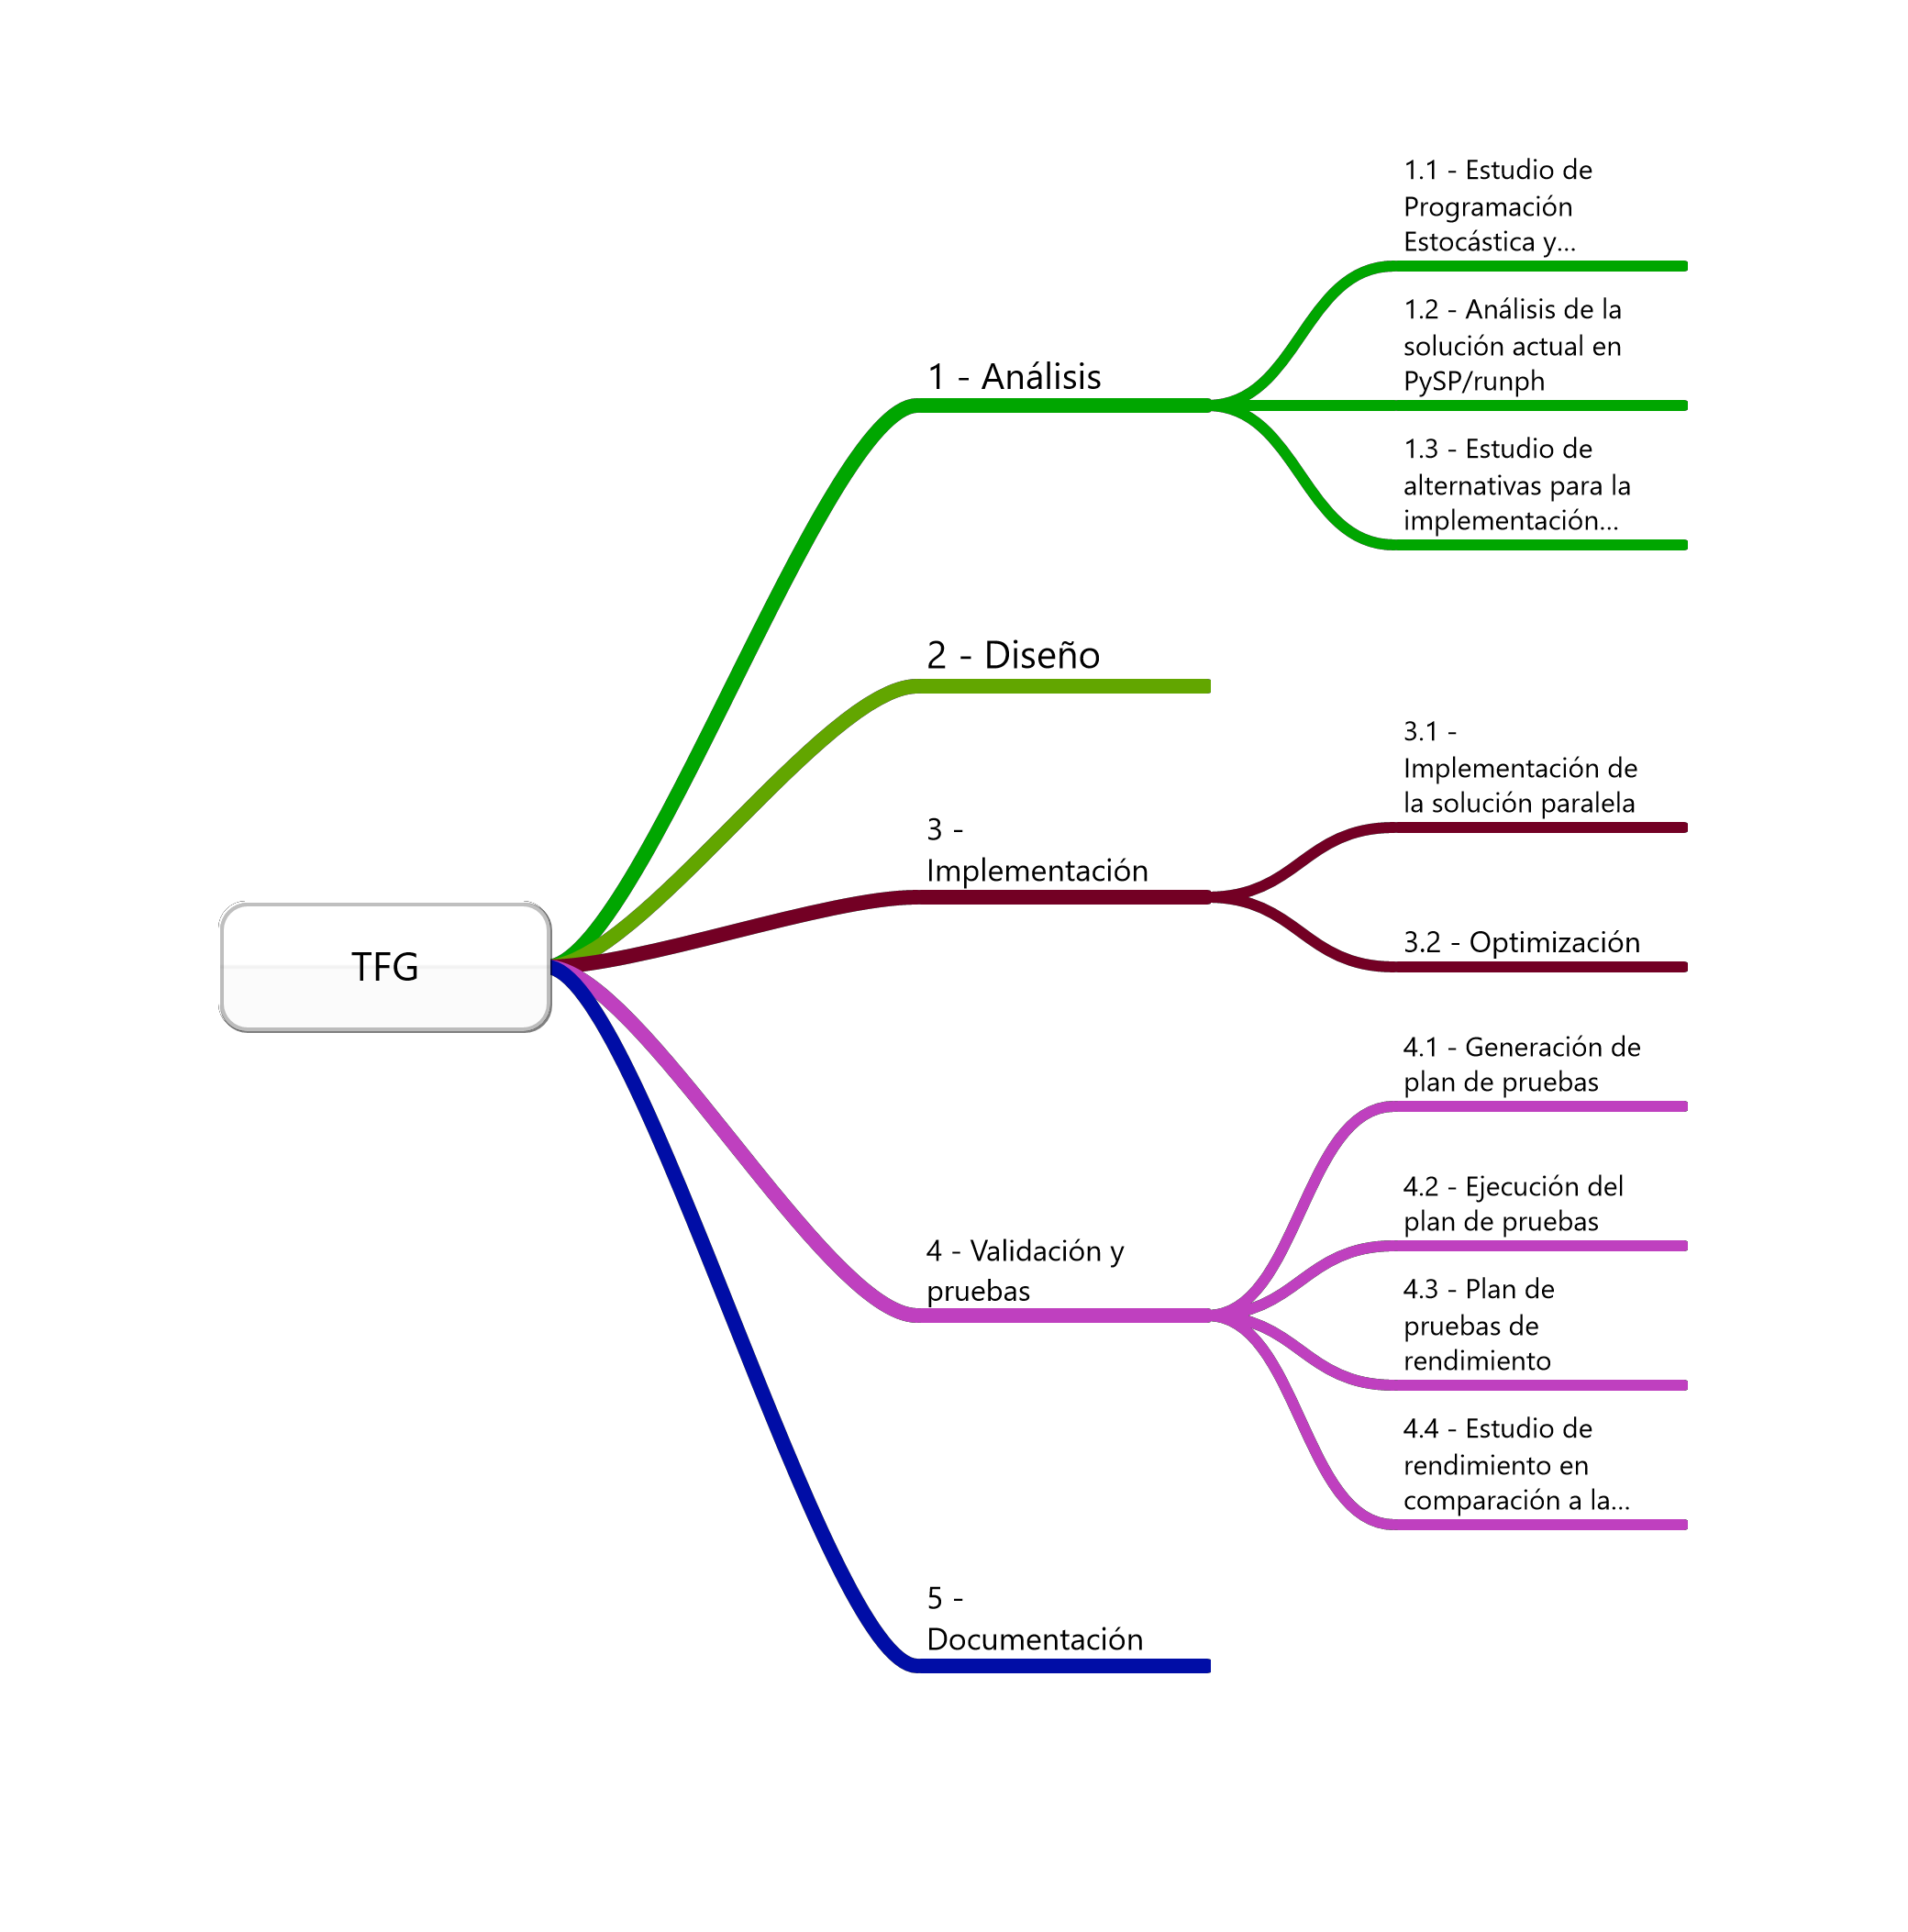
\includegraphics[width=9cm]{figuras/planificacion/edt-inicial.png}}
        \caption{EDT inicial}
    \end{figure}
\end{frame}

\begin{frame}[plain]
    \frametitle{Cronograma}
    \begin{figure}[H]
        \centerline{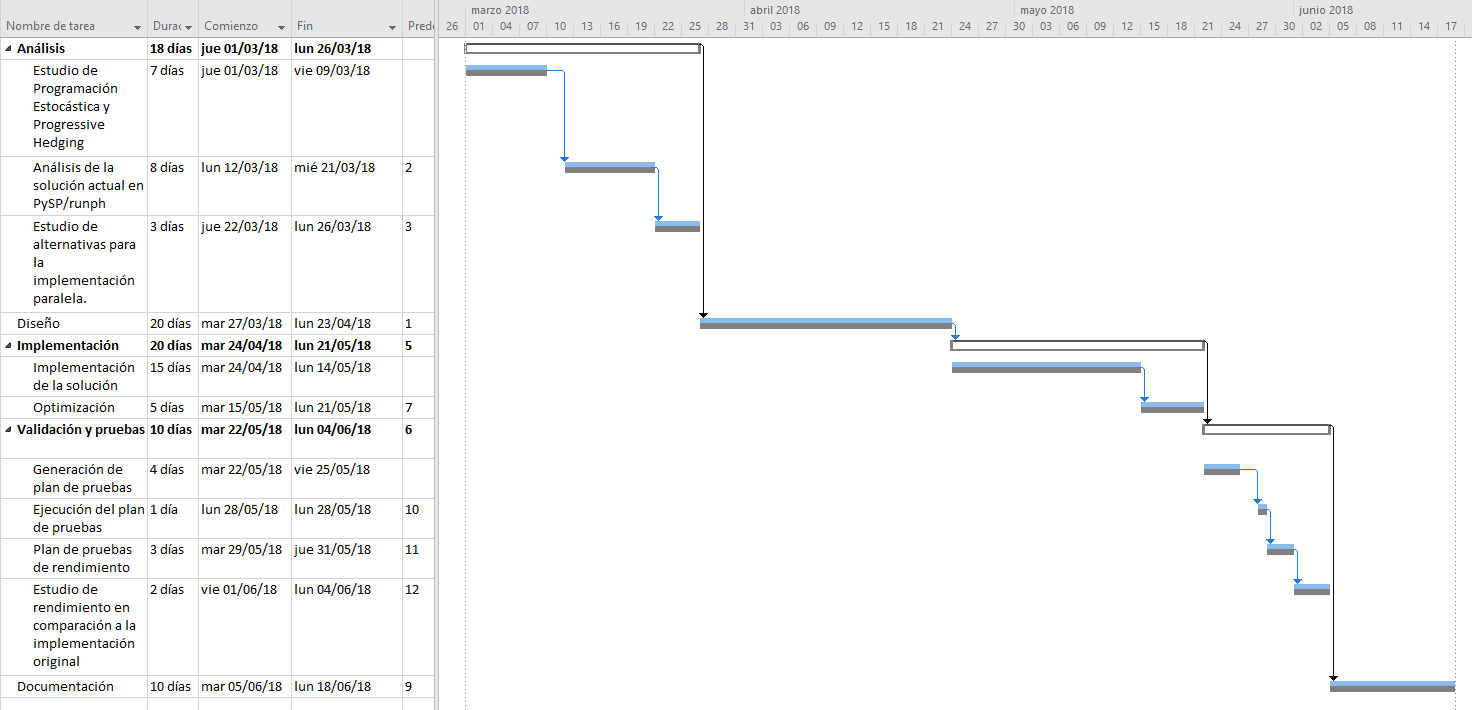
\includegraphics[width=12cm]{figuras/planificacion/linea-base.png}}
        \caption{Línea base}
    \end{figure}
\end{frame}

\begin{frame}[plain]
    \frametitle{Adaptación de la planificación}
    \begin{figure}[H]
        \centerline{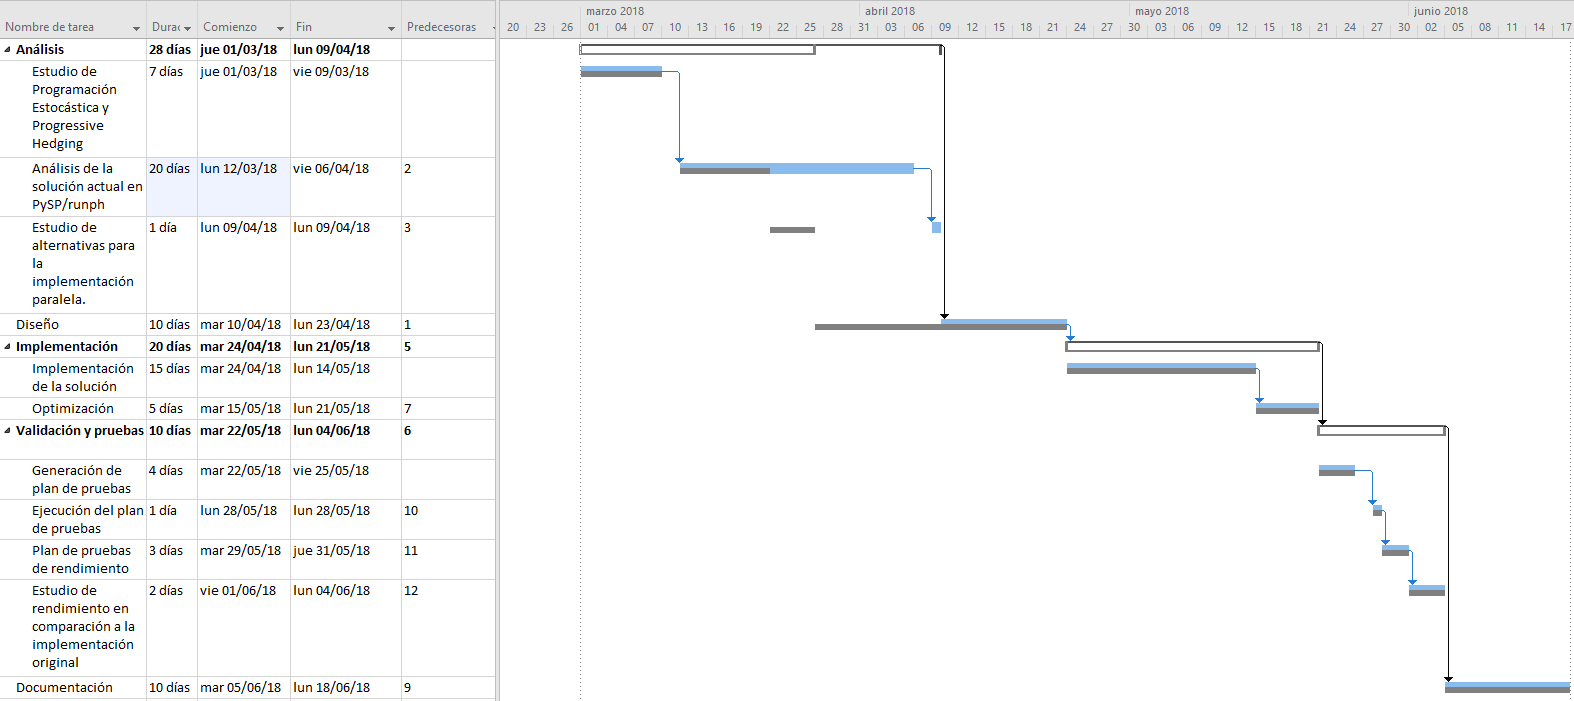
\includegraphics[width=12cm]{figuras/planificacion/1_retraso-analisis-inicial.png}}
        \caption{Primer retraso}
    \end{figure}
\end{frame}

\begin{frame}[plain]
    \frametitle{Adaptación de la planificación}
    \begin{figure}[H]
        \centerline{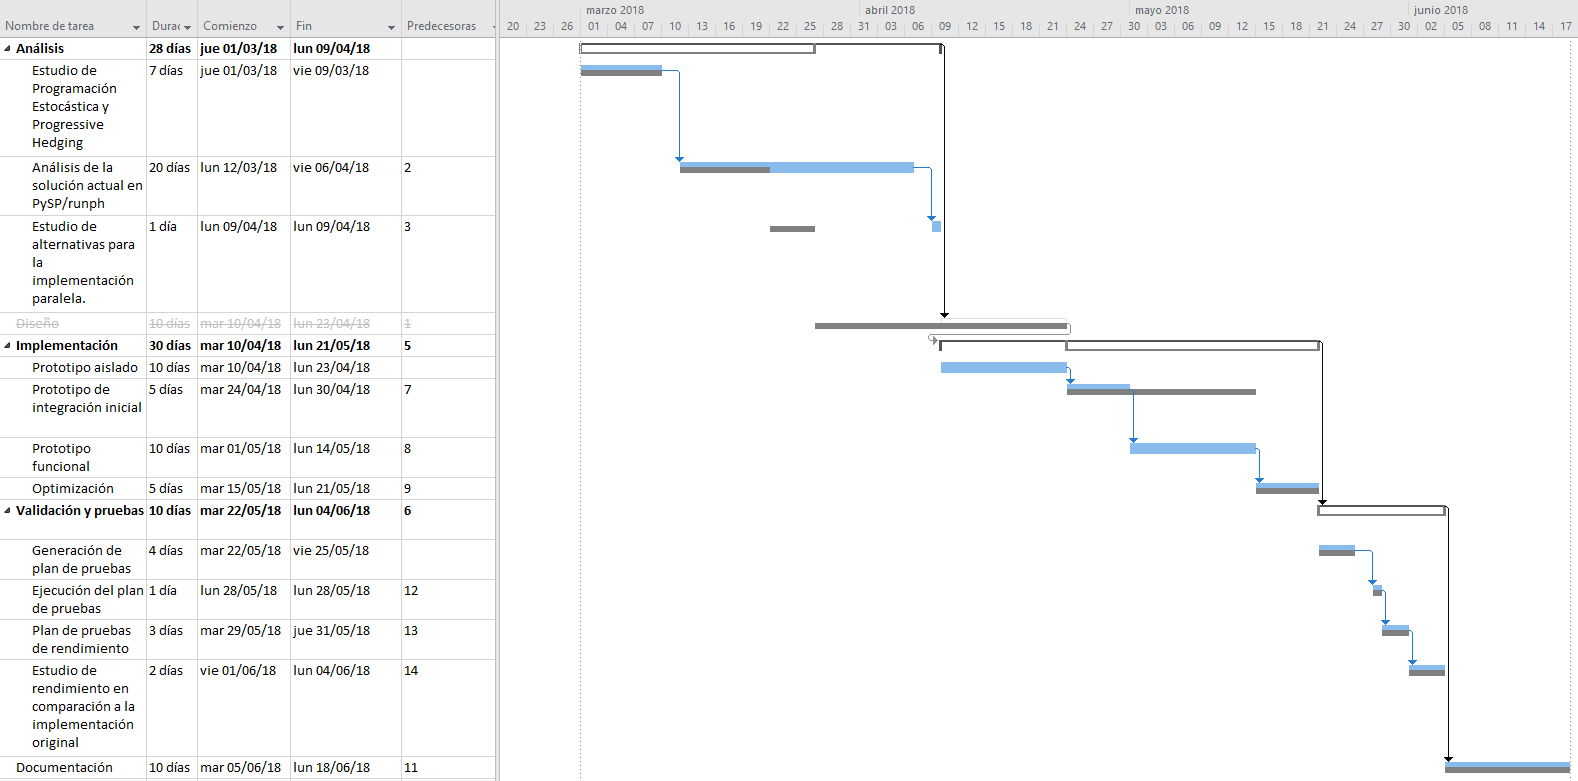
\includegraphics[width=12cm]{figuras/planificacion/2_linea-base-prototipos.png}}
        \caption{Línea base prototipos}
    \end{figure}
\end{frame}

\begin{frame}[plain]
    \frametitle{Cronograma final}
    \begin{figure}[H]
        \centerline{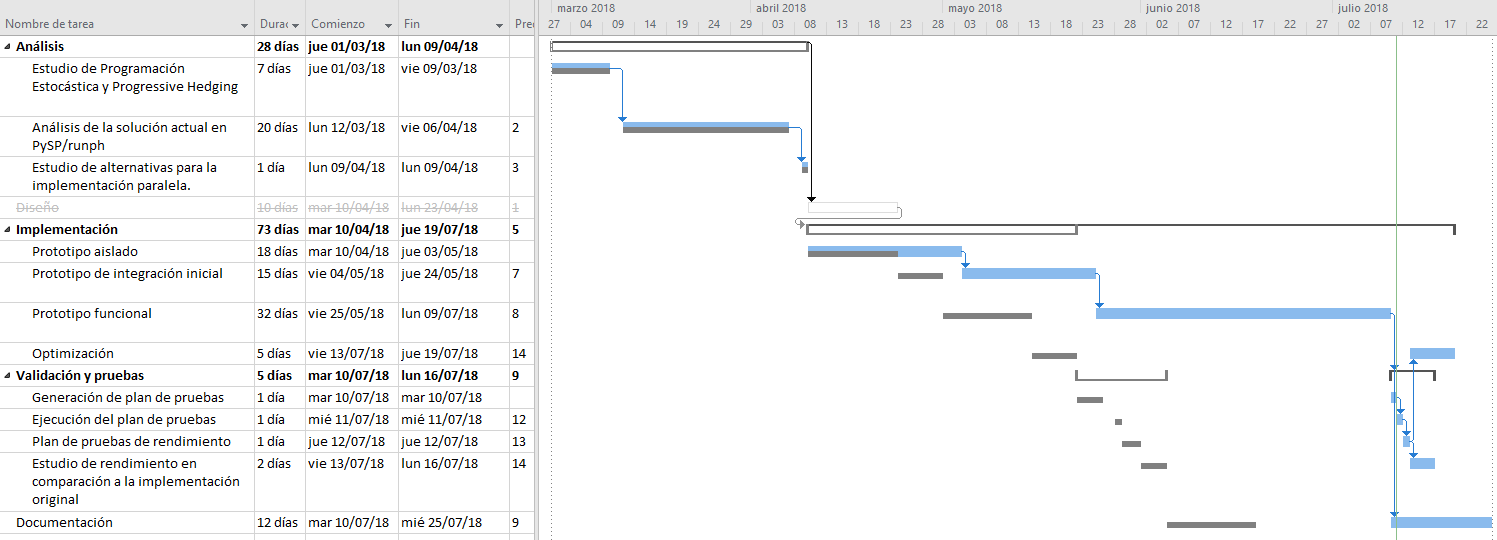
\includegraphics[width=12cm]{figuras/planificacion/3_linea-base-final.png}}
        \caption{Línea base final}
    \end{figure}
\end{frame}

\section{Análisis}

\subsection{Algoritmo \textit{Progressive Hedging}}

\begin{frame}
    \frametitle{\textit{Progressive Hedging}}
    \begin{itemize}
        \item Algoritmo iterativo
        \item Descomposición del árbol de escenarios en múltiples problemas lineales.
        \item Convergencia de las múltiples soluciones
    \end{itemize}
\end{frame}

\begin{frame}[plain]
    \frametitle{\textit{Progressive Hedging}}
    \begin{figure}[H]
        \centerline{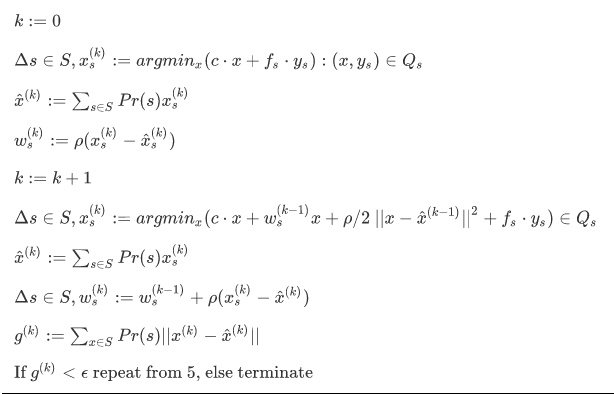
\includegraphics[width=12cm]{figuras/ph-pseudocode.png}}
        \caption{Pseudocódigo del algoritmo}
    \end{figure}
\end{frame}

\begin{frame}
    \frametitle{Implementación en Pyomo}
    \begin{enumerate}
        \item Se importan el modelo y los escenarios.
        \item Genera los objetos necesarios para la ejecución.
        % Solver manager, etc. Son configurables por el usuario.
        \item Cada iteración se divide en 3 fases:
        \begin{enumerate}
            \item ``presolve'': Preprocesa los escenarios.
            % Genera el archivo de entrada
            \item ``apply\_solver'': Ejecuta el solver externo.
            \item ``postsolve'': Adapta la salida del solver externo.
        \end{enumerate}
    \end{enumerate}
\end{frame}

\begin{frame}
    \frametitle{Implementación en Pyomo}
    \begin{itemize}
        \item Arquitectura basada en tareas
        \item Facilita intercambiar el módulo que ejecuta la solución del problema
        \item Simplifica la paralelización
    \end{itemize}
\end{frame}

\subsection{Herramientas}

\begin{frame}{}
    \frametitle{Herramientas}
    Para la nueva implementación paralela se analizarán dos posibles tecnologías:
    \begin{enumerate}
        \item Spark
        \item MPI
    \end{enumerate}
\end{frame}

\begin{frame}
    \frametitle{Spark}
    \begin{itemize}
        \item Herramienta Big Data de código abierto \pause
        \item Abstracción del entorno distribuido \pause
        \item Trabaja sobre RDD (\textit{Resilient Distributed Datasets}):
        \begin{itemize}
            \item Transformaciones
            \item Acciones \pause
        \end{itemize}
        \item Otros módulos (Dataframes, MLib, etc)
    \end{itemize}
\end{frame}

\begin{frame}{}
    \frametitle{MPI}
    \begin{itemize}
        \item Interfaz estándar de paso de mensajes
        \item Desacoplamiento entre trabajadores
        \item Implementación de bajo nivel (sincronización entre trabajadores, tipos personalizados)
        \item Funciones específicas para el tratamiento paralelo de datos (MPI\_BCAST, MPI\_SCATTER, etc)
    \end{itemize}
\end{frame}

\section{Diseño}

\begin{frame}[plain]
    \frametitle{Diseño}
    \begin{figure}[H]
        \centerline{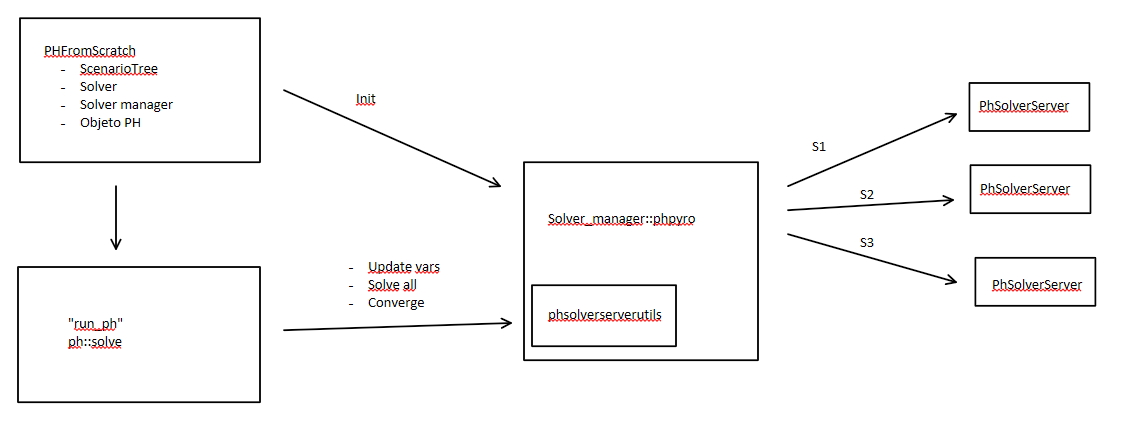
\includegraphics[width=12cm]{figuras/ph-diagram.png}}
        \label{fig:ph-diagram}
    \end{figure}
\end{frame}

\section{Implementación}

\begin{frame}{}
    \frametitle{Proceso}
    % Indicar que se hicieron prototipos, etc.
    \begin{itemize}
        \item Generación de 3 prototipos \pause
        \begin{enumerate}
            \item Prototipo inicial \pause
            \item Prototipo de integración \pause
            \item Prototipo funcional
        \end{enumerate}
    \end{itemize}
\end{frame}

\begin{frame}{}
    \frametitle{Funcionamiento-1}
    \begin{figure}[H]
        \centerline{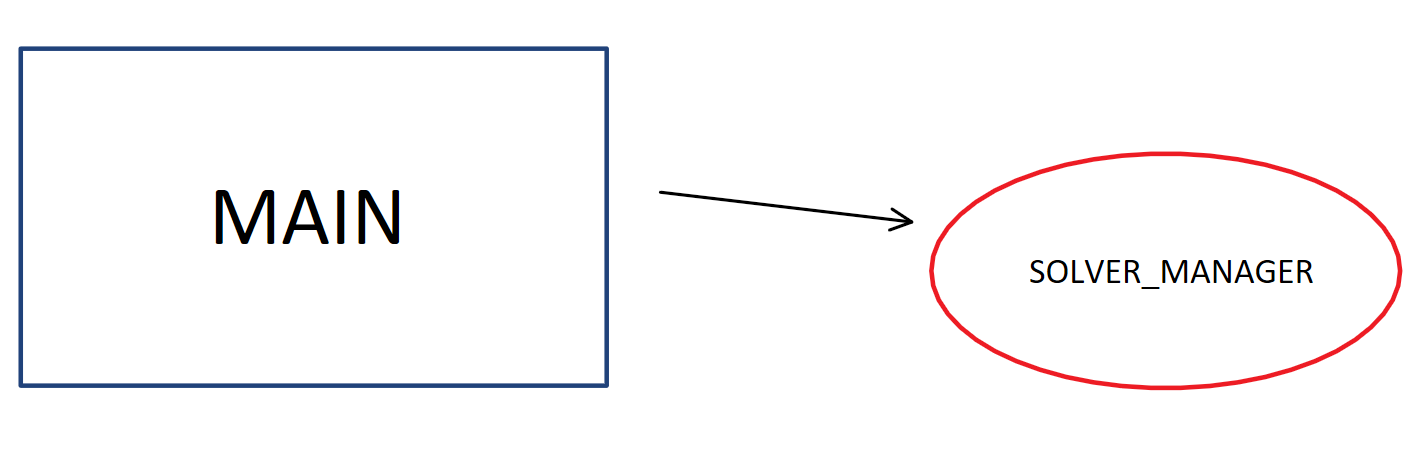
\includegraphics[width=12cm]{figuras/implementacion/impl-1.png}}
    \end{figure}
    % Dibujitos de cómo funciona la implementación de Spark
    % * Creación del RDD, es una lista y se inicializa en paralelo. 
    % * Envio del solver y cosas.
    % * Encapsulado de tareas, explicar el wrapper.
    % * Ver cómo se recogen los resultados. Explicar la naturaleza lazy, para ir encolando tareas.
\end{frame}

\begin{frame}{}
    \frametitle{Funcionamiento-2}
    \begin{figure}[H]
        \centerline{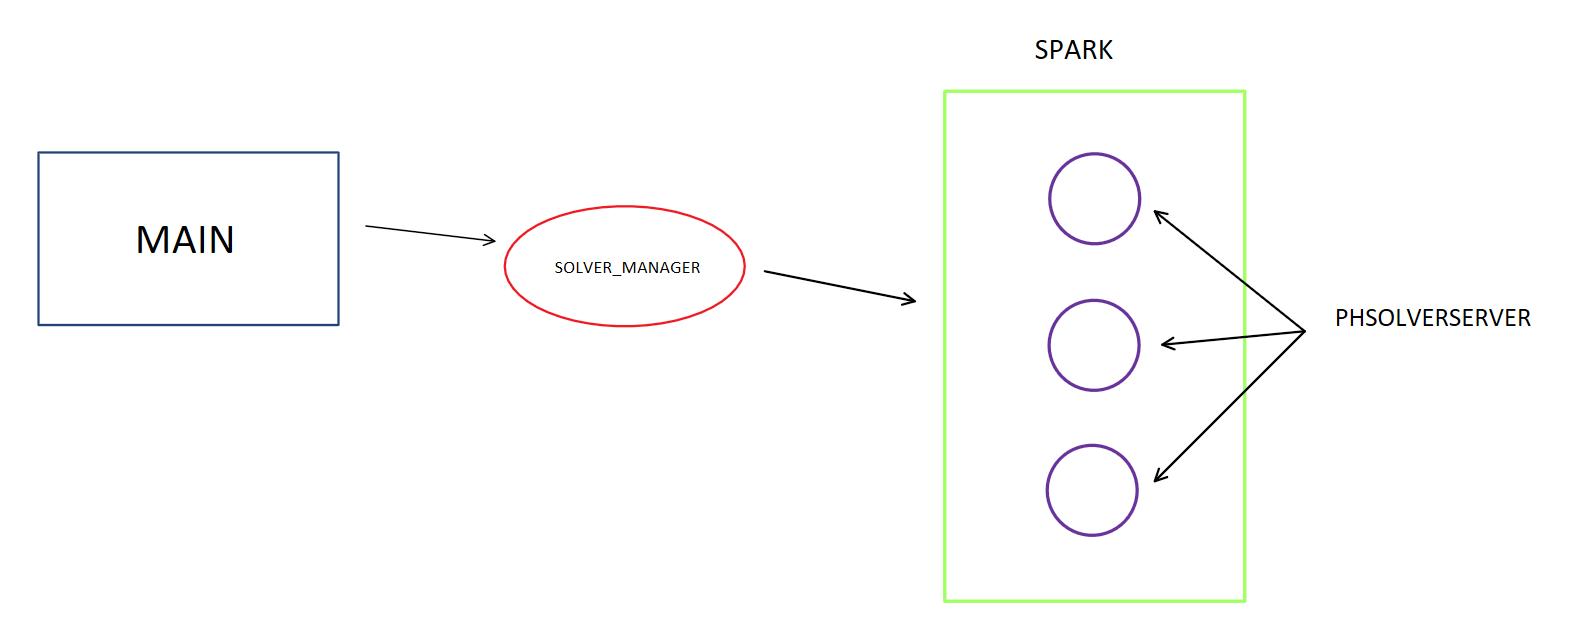
\includegraphics[width=12cm]{figuras/implementacion/impl-2.png}}
    \end{figure}
\end{frame}

\begin{frame}{}
    \frametitle{Funcionamiento-3}
    \begin{figure}[H]
        \centerline{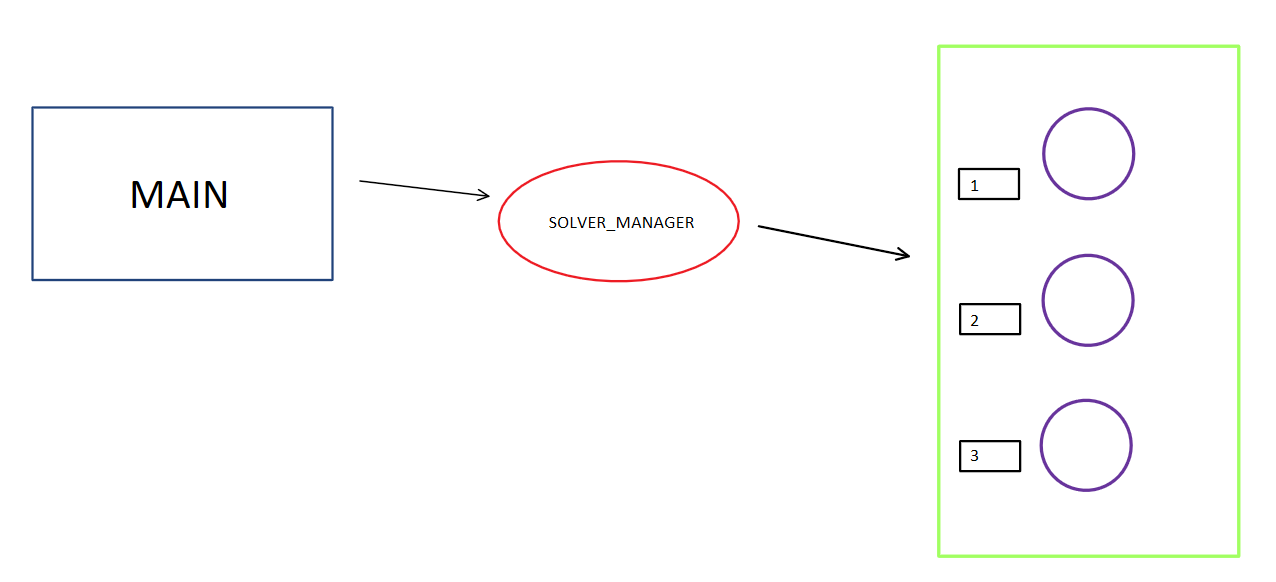
\includegraphics[width=12cm]{figuras/implementacion/impl-3.png}}
    \end{figure}
\end{frame}

\begin{frame}{}
    \frametitle{Funcionamiento-4}
    \begin{figure}[H]
        \centerline{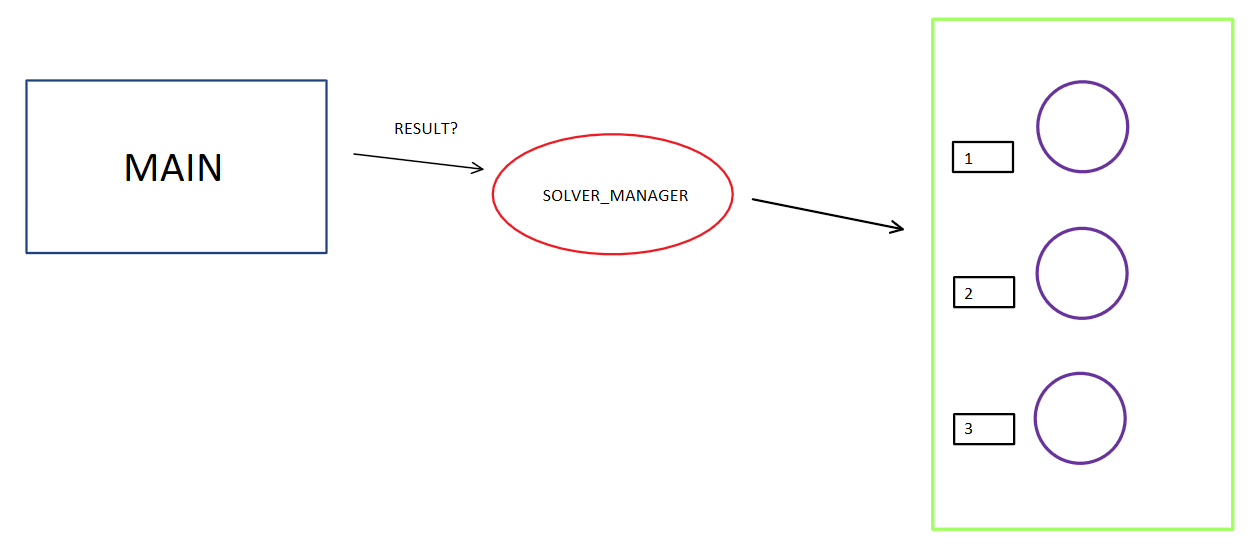
\includegraphics[width=12cm]{figuras/implementacion/impl-4.png}}
    \end{figure}
\end{frame}


\begin{frame}{}
    \frametitle{Funcionamiento-5}
    \begin{figure}[H]
        \centerline{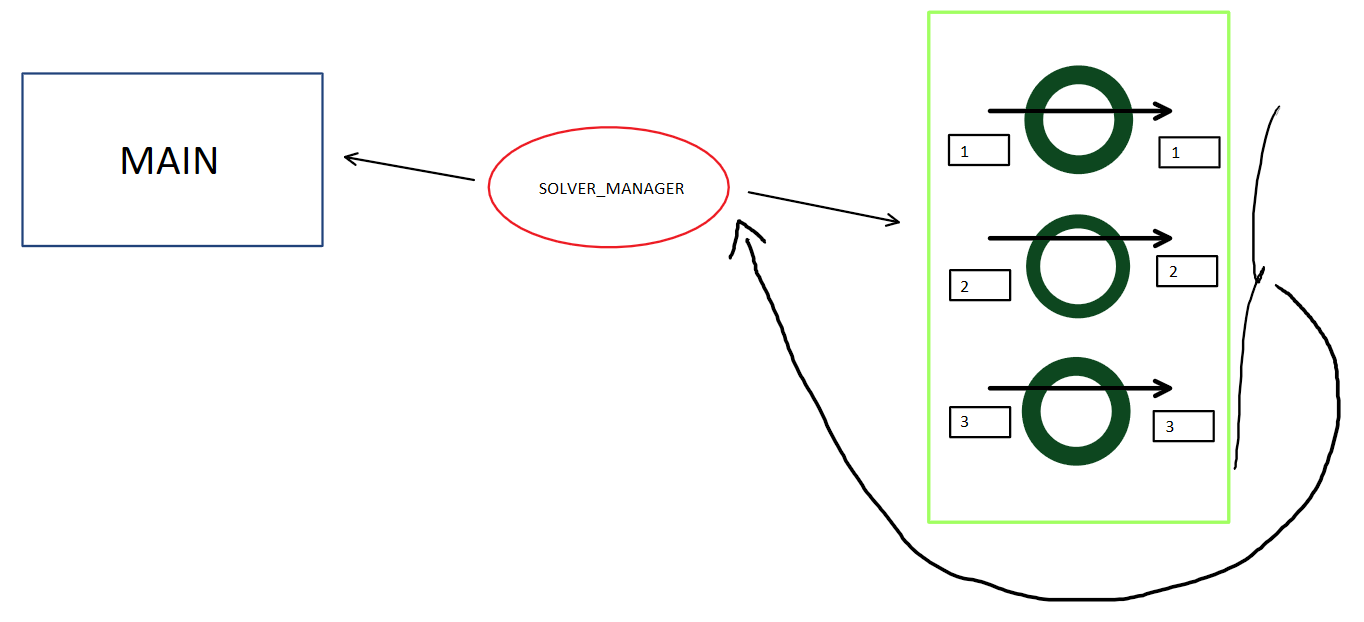
\includegraphics[width=12cm]{figuras/implementacion/impl-5.png}}
    \end{figure}
\end{frame}

\section{Pruebas}

\begin{frame}{}
    \frametitle{Pruebas}
    \begin{itemize}
        \item Diseño de pruebas funcionales
        \begin{itemize}
            \item Diferentes opciones de configuración que modifican la ejecución
            \item Resolución de los ejemplos
        \end{itemize}
        \item Diseño de pruebas de rendimiento
    \end{itemize}
\end{frame}

\begin{frame}{}
    \frametitle{Recursos}
    % Indicar que también se hicieron pruebas funcionales, pero para la presentación nos interesa el rendimiento, como objetivo principal del proyecto.
    % Decir que se usaron los ejemplos que vienen y ya.
    \item Se probarán los ejemplos \textit{Finance} y \textit{Hydro}
    \item Se prueba la escalabilidad en 1 y 8 hilos
    \item Se medirá el tiempo total de ejecución y el tiempo medio por iteración
\end{frame}

\begin{frame}[plain]
    \frametitle{Resultados}
    \begin{figure}[H]
        \centerline{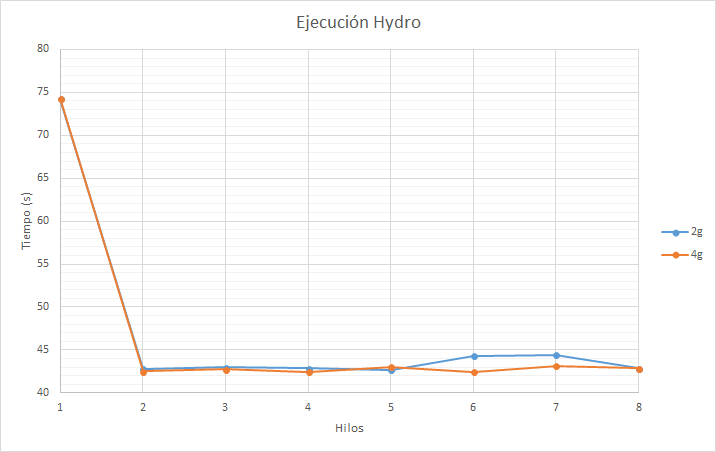
\includegraphics[width=13cm]{figuras/pruebas/test-hydro.png}}
        \caption{Tiempos de ejecución Hydro con múltiples hilos con 2GB o 4GB}
        \label{fig:test-hydro}
    \end{figure}
\end{frame}

\begin{frame}[plain]
    \frametitle{Resultados}
    \begin{figure}[H]
        \centerline{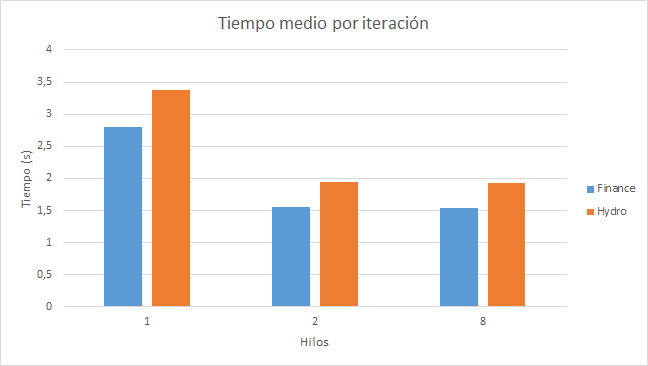
\includegraphics[width=13cm]{figuras/pruebas/test-iteration-time.png}}
        \caption{Tiempo medio por iteración}
        \label{fig:test-iteration-time}
    \end{figure}
\end{frame}

\section{Conclusiones}

\begin{frame}{}
    \frametitle{Conclusiones}
    \begin{itemize}
        \item Extensibilidad de las herramientas Big Data y Spark en concreto \pause
        \item Integración satisfactoria con Pyomo \pause
        % La arquitectura implementada en Pyomo permite que el nuevo módulo funcione como si hubiese sido integrado desde un principio.
        \item Escalabilidad conseguida
        % Los valores de escalabilidad son prometedores. Aunque el overhead de spark es importante, tenemos que tener en cuenta que tampoco ejecutamos las pruebas en un entorno realista
    \end{itemize}
\end{frame}

\begin{frame}{}
    \frametitle{Lecciones aprendidas}
    \begin{itemize}
        \item Importancia de la planificación \pause
        \begin{itemize}
            \item Uso de un ciclo de vida adecuado
            \item Tener en cuenta el tiempo de formación cuando se usan nuevas herramientas \pause
        \end{itemize}
        \item Adaptación de una arquitectura orientada a objetos a Spark \pause
        \item Herramientas de gestión de la configuración y planificación \pause
    \end{itemize}
\end{frame}

\begin{frame}{}
    \frametitle{Trabajo futuro}
    \begin{itemize}
        \item Pyomo es Open Source \pause
        \item Entorno de pruebas adecuado
        \item Mayor optimización en el uso de Spark
    \end{itemize}
\end{frame}

\begin{frame}[plain]
    \titlepage
\end{frame}

\end{document}

